% MIT License

% Copyright (c) 2022 Mihdí Caballero

% Permission is hereby granted, free of charge, to any person obtaining a copy
% of this software and associated documentation files (the "Software"), to deal
% in the Software without restriction, including without limitation the rights
% to use, copy, modify, merge, publish, distribute, sublicense, and/or sell
% copies of the Software, and to permit persons to whom the Software is
% furnished to do so, subject to the following conditions:
%
% Based on article class and in spanish language by default
\documentclass[a4paper,12pt,english]{article}
% Load all packages and settings in the preamble 
% *** LANGUAGE PACKAGES ***
%\usepackage[es-nodecimaldot, mexico]{babel} 
\usepackage[utf8]{inputenc}
\usepackage[T1]{fontenc}
\usepackage{lmodern}		% Great font
\renewcommand*\familydefault{\sfdefault}
\usepackage[useregional]{datetime2}		% To use several date formats
\usepackage{lipsum}		% For dummy text

% *** GEOMETRY PACKAGES ***
\usepackage{geometry}
\geometry{left=25mm,
	right=25mm,
	top=22mm,
	bottom=35mm,
	headheight = 0 mm,
        footskip=10mm  
} 
\usepackage{lastpage}

% *** COLOR PACKAGES ***
\usepackage[table]{xcolor}		% "table" for table rowcolors
% Color definitiions
\definecolor{blue}{RGB}{0,89,140}
\definecolor{gray}{RGB}{242,242,242}
\definecolor{grayblack}{RGB}{50,50,50}
\definecolor{blue2}{RGB}{10,62,157}
\definecolor{red2}{RGB}{173,17,0}
\definecolor{gray2}{RGB}{230,230,230}

% *** HEADING AND FOOTER ***
\usepackage{fancyhdr} % For heading and footers
% \renewcommand{\headrulewidth}{0.01pt}
% \let\oldheadrule\headrule% Copy \headrule into \oldheadrule
% \renewcommand{\headrule}{\color{blue}\oldheadrule}% Add colour to \headrule
\renewcommand{\footrulewidth}{0.9pt} 
\let\oldfootrule\footrule%
\renewcommand{\footrule}{\color{blue}\oldfootrule}% Add colour to \headrule
\pagestyle{fancy}         % Default page style
\fancyhf{}
\renewcommand{\headrulewidth}{0pt}

%\cfoot{}                             % Empty foot center  
% \lhead{}
% \chead{}
% \rhead{}
%\lhead{\includegraphics[width=0.15\textwidth]{logo}}     
%\chead{\textcolor{grayblack}{\author}}
% \rhead{\textcolor{grayblack}{\DTMsetstyle{ddmmyyyy} \date}}
\lfoot{\textcolor{grayblack}{\small User's Manual} }
\cfoot{\textcolor{grayblack} {aiirmap}}
\rfoot{\textcolor{grayblack}{\small Pg. \thepage} }
%\setlength{\footskip}{12pt}

% *** GRAPHICS RELATED PACKAGES ***
\usepackage{graphicx}       % Loading images
\usepackage{float}          % Figures inside minipages
\usepackage{wrapfig}		% Text wrapped around figure
\usepackage{tikz}			% Used to load cover figure
\usepackage[hypcap,font={color=grayblack}]{caption} % used to style the captions
\usepackage{subcaption} 	% For subfigures
\usepackage{overpic}		% To add text over figures
\graphicspath{{././figures/}}  % Figures relative directory

% *** TITLE PACKAGES ***
\usepackage{titlesec}
\titleformat{\section}{\color{blue}\normalfont\Large\bfseries}{\thesection}{1em}{}
\titleformat{\subsection}{\color{blue}\normalfont\large\bfseries}{\thesubsection}{1em}{}
\usepackage{setspace} % Para ajustar la separación entre líneas del documento

% *** TABLE PACKAGES ***
\usepackage{booktabs}
\usepackage{colortbl}
\usepackage{footnote} % To have footnotes inside tables
\usepackage{array}

\usepackage{xurl} % Lo cargo antes de hyperref, porque ese ya lo carga también.
\urlstyle{sf} % Estilo de los url pasa a Sans Serif.



%%% EQUATIONS %%%
\usepackage{mathtools}

\usepackage[
backend=biber,	% Backend para las referencias (no modificar)
style=numeric, 		% Estilo APA de bibliografía
sorting=none,		% Para tener ordenadas las citas
natbib=true,	% Utiliza natbib
url=true, 		% Para que aparezca o no la url
doi=true,		% Para que aparezca o no el DOI
isbn=false 		% Para que aparezca o no el ISBN
]{biblatex}
\addbibresource{biblio.bib}


\usepackage[colorlinks,
citecolor=cyan,
urlcolor=blue,
linkcolor=blue,
citebordercolor={0 0 1},
urlbordercolor={0 1 1},
linktocpage,
hyperfootnotes=true
]{hyperref}
\renewcommand{\sectionautorefname}{Section}
\renewcommand{\subsectionautorefname}{Section}
\renewcommand{\subsubsectionautorefname}{Section}
\renewcommand{\figureautorefname}{Figure}
\renewcommand{\tableautorefname}{Table}
\renewcommand{\equationautorefname}{Equation}
\renewcommand{\itemautorefname}{Item}
\renewcommand{\pageautorefname}{Page}

\begin{document}
	% Cover page
	\begin{titlepage}
    % Vertical spacing to push image ~2/5 down
    \thispagestyle{empty} % No header nor footer
    \vspace*{0.15\textheight}

    % Centered image
    \begin{center}
        
\includegraphics[width=0.8\textwidth]{aiirmap_logo_cropped} % Replace with your image filename
    \end{center}
    
    % Subtitle below image
    \vspace{-1em}
    \begin{center}
        {\Huge \textbf{A Framework for}}\\[0.7em]
        {\Huge \textbf{Machine Learning Enhanced}}\\[0.5em]
        {\Huge \textbf{Design}}

        
    \end{center}
    
    % Push remaining content to bottom
   \vspace*{0.2\textheight}
    
    % Bottom text
    \begin{center}
        \begin{spacing}{2}
				{\Huge \bfseries User's Manual} \\ [0.5cm]
				{\Large Robert F. H. Hunter} \\
				{\Large August 2025, v1}
		\end{spacing}
    \end{center}
    
    % \thispagestyle{empty} % No header nor footer
	
	% 	
\includegraphics[width=21cm]{aiirmap_logo_cropped}
	
	% \hfill 
	% %	Title
	% \begin{minipage}{8cm}
	% 	\vspace{5cm} 
	% 	\begin{flushright}
	% 		\begin{spacing}{3}
	% 			{\fontsize{50}{60}\selectfont aiirmap\\
 %                \fontsize{25}{35}\selectfont A Framework for Machine Learning Enhanced Design}
	% 		\end{spacing}
	% 	\end{flushright}
	% \end{minipage}
	% \vfill 
	% \hfill
	% % Subtitle, author and date
	% \begin{minipage}{10cm}
	% 	\begin{flushright}	
	% 		\begin{spacing}{2}
	% 			{\Huge \bfseries User's Manual} \\ [0.5cm]
	% 			{\Large Robert F. H. Hunter} \\
	% 			{\Large August 2025, v1}
	% 		\end{spacing}
	% 	\end{flushright}
	% \end{minipage}
\end{titlepage}

	\newpage             
	\tableofcontents      
	\newpage

    \section{Overview} \label{overview}
    aiirmap is available as a github repo: 
    \url{https://github.com/rfhhunter/aiirmap} \\
    
    aiirmap is a codebase which interfaces simulation softwares with Python databasing, machine learning, and optimization capabilities. It was originally designed to couple optoelectronic device simulations in Synopsys Sentaurus TCAD \cite{tcad} with principle component analysis \cite{pca1, pca2} dimensionality reduction. It is written to be easily extendable to new simulation softwares and machine learning methods. To ease adoption, aiirmap is built upon standard Python packages; such as pandas \cite{pandas1, pandas2}, scikit-learn \cite{sklearn}, tensorflow \cite{tensorflow}, scipy \cite{scipy}, numpy \cite{numpy}, and matplotlib \cite{matplotlib}. \\
    
    The basic functionality of aiirmap is as a databasing tool. Large sets of experiments can be easily defined using pandas DataFrame based \textit{DataBases}. They are sent to and collected from the simulation softwares, manipulated (split, merged, sorted, thresholded, cleaned, etc.), subjected to machine learning, and analyzed with user-defined runfiles. This highly versatile run paradigm facilitates comprehensive design of experiments and problem space exploration. It also empowers machine learning approaches which hinge upon large datasets and flexible, reliable data pipeline control. \textit{DataBases} and machine learning instances are saved for later use with csv and pickle format, respectively.   \\         

    The remainder of this document is organized as follows: \autoref{run} provides an operational overview including install and setup (\autoref{setup}), an outline of the project structure (\autoref{structure}), the basic aiirmap objects (\autoref{objects}), and an outline of the runfile paradigm (\autoref{runfiles}). \autoref{softwares} describes how aiirmap interacts with simulation softwares such as Synopsys Sentaurus TCAD (\autoref{tcad}). \autoref{ml} discusses implementation of  machine learning algorithms in the aiirmap code. \autoref{new} gives instructions on how to include new simulation softwares and machine learning functionalities. \autoref{notes} provides some anecdotal notes on running aiirmap. Finally, in \autoref{pubs} is a list of publications which employ aiirmap and, in \autoref{ack}, persons and entities who contributed to the development of aiirmap are gratefully acknowledged. \\  
    
    Issues with the code or documentation can be reported in the github repository.\\
    

    \section{Running aiirmap} \label{run}
    This section overviews how to install and setup aiirmap (\autoref{setup}). It then outlines the project structure (\autoref{structure}) and custom objects (\autoref{objects}) to give context to the run paradigm (\autoref{runfiles}), which is built around user-defined "runfiles". \\
    
    \subsection{Install and Setup} \label{setup}
    "Installation" of aiirmap is straightforward. Retrieve the aiirmap project from the github repo (\url{https://github.com/rfhhunter/aiirmap}) and clone it to your machine. aiirmap uses Python 3. The specific version is restricted only by the requirements of the packages that it uses. It has been verified on Python 3.9, 3.11, 3.12, and 3.13. The remainder of the aiirmap installation is to install any Python packages it includes, if you do not have them already. The majority of these are listed at the top of the \textit{aiirmapCommon.py} file. No specific versioning of the included Python packages is required. aiirmap operation is verified with up-to-date packages at the time of the writing of this document (Aug. 2025). \\

    Setup of aiirmap is likewise very easy. All aiirmap requires is a folder with three subfolders to save output files. This folder is referred to as the filing folder. It can be located anywhere which is read-write accessible while running the codebase. In aiirmap its location is defined in \textit{config.py} using the variable \textit{filingdir}. Filing folder subfolders are used to organize the output files. Defined immediately below \textit{filingdir} in \textit{config.py} they include a folder for databases and machine learning instance pickles (\textit{dbdir}), copies of simulation files (\textit{sfdir}), and plots (\textit{pldir}). No other setup is required to run aiirmap. The remaining variables in \textit{config.py} set the defaults for other aspects of the codebase, as described below. \\      
    
    \subsection{Project Structure} \label{structure}
    This section gives a very brief overview of the project structure, primarily to give context to the runfiles paradigm. For more information on the functions and code architecture please refer to the extensive comments in the code itself. \\

    The main folder of aiirmap contains the files with configuration variables (\textit{config.py}), an import file (\textit{aiirmapCommon.py}), bash terminal wrappers for a few of the functions (\textit{pyDBCollector.py, pyProjectCollector.py, grid-runner.py}), and the files for creating Sentaurus command files (\textit{py<2/3>prepper.py}).\\

    Several subfolders exist. The \textit{utilities} folder contains the heart of aiirmap functionality. Functions are the  split topically into different files with relevant names. The \textit{runfiles} folder is the location where users can drop their control scripts. A couple example runfiles are included in the aiirmap repository. The \textit{user\_manual} folder contains the latex files for this document. And the \textit{archive} offers a location to drop old files for safekeeping.\\
    
    
    \subsection{Project Objects} \label{objects}
    There are two main aiirmap objects; \textit{DataBases} and \textit{aiirMappings}. These objects are substantiated as Python classes located in the files \textit{utilities/databasing.py} and \textit{utilities/ml/machine\_learning.py}, respectively. This section briefly overviews their intended operation and attributes. For further details please refer to comments in the py files.\\

    \subsubsection{DataBases}
    aiirmap \textit{DataBases} are how sets of simulations are realized in the code. They are defined in the file \textit{utilities/databasing.py} and this is also where all the functions for their creation and manipulation are located. The aiirmap \textit{DataBase} is based upon the \href{https://pandas.pydata.org/docs/reference/api/pandas.DataFrame.html}{pandas DataFrame} allowing large datasets to be easily and quickly defined and manipulated (cleaned, split, combined, sorted, thresholded, etc.). aiirmap \textit{DataBases} are saved as csv files in the database filing folder for later use. Their attributes are as follows, provided in the order they appear in the csv file:
    
    \begin{itemize}
    \item \textbf{grid} [boolean]:\\
    Whether or not the \textit{DataBase} includes only simulation inputs. This is determined by whether or not the \textit{experiment-outputs} column exists in the \textit{DataBase.dataframe} (see below for more information). \textit{DataBases} with only reference and/or simulation input columns are referred to as "Grids". The first line in a \textit{DataBase} csv is the comment "\#AiirMap DataBase". The next line will contain the text "GRID FILE" if the \textit{DataBase} is a Grid or will be empty if not.  
    \item \textbf{dbfilename} [string ending in .csv]:\\
    The identifier for the dataset; its filename. One line in the csv file.
    \item \textbf{dbFile} [path string]:\\
    The path to the dataset. Note that this does \textit{not} need to match its actual location on your machine, when a \textit{DataBase} is loaded the accurate \textit{dbFile} will be used in the code (and will be recorded if the \textit{DataBase} is saved). One line in the csv file.
    \item \textbf{lineage} [list with format of [[datetime string, action description str], ...]]:\\
    A recording of past manipulations of the \textit{DataBase}. This is saved in the csv file using multiple lines; one line for each entry in the list with a header line reading "Lineage:". Lineage inheritance is also implemented. For \textit{DataBases} created through merging of other \textit{DataBases} a few lines of the lineage of these ancestors is recorded in the new database csv file and distinguished by >>>> and <<<< (the size of the inherited lineage can be set in \textit{config.py}). 
    \item \textbf{dataframe} [\href{https://pandas.pydata.org/docs/reference/api/pandas.DataFrame.html}{pandas DataFrame}]:\\
    The main attribute for the \textit{DataBase}. This is where your dataset data goes. Simulation inputs and outputs are given by the columns and are typically indexed with text (for instance with the parameter and variable names used in a Synopsys Sentaurus TCAD model). Different experiments (simulation instances) are given by the rows and are indexed with integers. The \textit{DataBase.dataframe} has two special columns which act to separate the dataframe into three sections; reference, inputs, and outputs. These two columns are defined as \textit{experiment-inputs} and \textit{experiment-outputs} (this default can be changed or added to by editing \textit{<in/out>putStartStrs} in \textit{config.py}). They are placed at the left-side of each section resulting in a column structure which looks like; \textit{db\_idx}|reference columns|\textit{experiment-inputs}|input parameter columns|\textit{experiment-outputs}|output variable columns (where \textit{db\_idx} is the dataframe index). Note that \textit{db\_idx} begins at 0, while \textit{experiment-<in/out>puts} begin at 1 (are the experiment number rather than its index).
    \end{itemize}\\

    \subsubsection{aiirMappings}
    \textit{aiirMappings} are the objects which codify instances of machine learning application when data is transformed. They include the inputs and outputs to the machine learning algorithm as well as the mapping between them. Information on which algorithm has been employed and how (its hyperparameters) are also recorded here. The \textit{aiirMapping} class is defined in the file \textit{utilities/ml/machine\_learning.py}. \textit{aiirMappings} are saved using the pickle (.pkl) binary file format. The attributes of the \textit{aiirMapping} object, in the order given in the code, are as follows:

    \begin{itemize}
    \item \textbf{mapType} [(a specific) string]:\\
    The label for the machine learning algorithm which was used. The labels for the implemented algorithm are \textit{pca} and \textit{ae}. \textit{pca} is the label for principle component analysis, a linear dimensionality reduction technique \cite{pca1, pca2}. \textit{ae} is the label for nonlinear dimensionality reduction using autoencoder architecture neural nets \cite{ae}.
    \item \textbf{mapName} [string]:\\
    Descriptor for the \textit{aiirMapping} instance. As opposed to \textit{DataBase.dbfilename} this string should not end in .pkl. 
    \item \textbf{mapFolder} [string path]:\\
    The path to the folder containing the \textit{aiirMapping} pickle file. Note that this does \textit{not} need to match the actual location of the pickle file in the code, when the \textit{aiirMapping} is loaded then the accurate location is used in the code and will be written to file if the \textit{aiirMapping} is saved. 
    \item \textbf{settings} [dictionary]:\\
    These are the hyperparameters for the given machine learning algorithm. Each algorithm has different hyperparameter options and thus different \textit{settings} dictionary structure. For the \textit{aiirMapping.settings} structures specific to each algorithm see the comments at the top of the \textit{aiirMapping} class definition.
    \item \textbf{ml} [machine learning object]:\\
    Also located in \textit{utilities/ml/machine\_learning.py} is the definition of classes for each type of machine learning algorithm (so far only \textit{DimensionalityReduction}). These objects package the actual machine learning objects created by the scikit-learn or tensorflow (or other package) functions for later access.
    \item \textbf{filteredInputDB} [DataBase]:\\
    This is the aiirmap \textit{DataBase} with the input data for the machine learning algorithm. Filtering refers to the fact that the experiments in this dataset have been cleaned and thresholded, it contains only the data which is actually being used as input to the algorithm. This \textit{DataBase} contains all columns present in the original \textit{DataBase} for this filtered data.
    \item \textbf{filteredInputGrid} [(Grid) DataBase]:\\
    Very similar to the previous attribute but now the reference and outputs columns have been removed. Input columns which are extraneous to the machine learning training have also been removed in a process called column cleaning (see the function \textit{dbDRCleanCols} in \textit{utilities/databasing.py} for more information). This is the training data (only).  
    \item \textbf{results} [dict]:\\
    The outputs from the machine learning algorithm. Each algorithm will have different outputs according to type and intended operation. For the \textit{aiirMapping.results} structures specific to each algorithm see the comments in the \textit{aiirMapping} class definition.
    
    \end{itemize}\\
    
    \subsection{Runfiles} \label{runfiles}
    aiirmap provides the functions and objects for a versatile simulation flow control. It is up to the user how to they want to use this functionality and, indeed, the exploratory nature of design and machine learning enhanced design means that this use will evolve. "Runfiles" are simply the user scripts written to access aiirmap functionality. Users may also directly use the Python terminal if they prefer. All aiirmap capabilities are imported by including \textit{aiirmapCommon.py} at the start of your script (\textit{from aiirmapCommon import *}). \\

    Typical runfile operations are listed below. These are just examples offered to spark the user's imagination. Any desired functionality can be included in runfiles and organized as the user sees fit. Runfile functions may also be loaded as modules into other runfiles. General useful functionality can be ported into the aiirmap utilities and shared if the user wishes.   \\
    
    Potential runfile operations: Creating a new \textit{DataBase} and filling it with data to send as input to the simulation software. Creating a new \textit{DataBase} from one or more other \textit{DataBases}. Loading a \textit{DataBase} and running analysis or machine learning and potentially outputting a new \textit{DataBase} for further simulation. Comparing performance across \textit{DataBases}. Designing specific investigations. Creating sequential simulation run operations. etc. \\  


    \section{Simulation Software Interactions} \label{softwares}
    This section outlines how aiirmap interacts with the simulation softwares which have been implemented in its environment. As mentioned, aiirmap has been designed in a manner which allows it to be extended to include other simulation softwares.  The procedure for adding new softwares into the code is outlined in \autoref{new} below. Users may add subsections here outlining their software interface. \\
    
    \subsection{Synopsys Sentaurus TCAD Interaction} \label{tcad}
    Synopsys Sentaurus TCAD is an finite element analysis optoelectronics device simulator \cite{tcad}. aiirmap was originally written to interface Python with Sentaurus to provide databasing and machine learning capabilities. Sentaurus interacts with Sentaurus in two ways; collection of simulation results and (batch-capable) run control. \\

    Collection of results is instantiated in the Sentaurus project flow using the Sentaurus Python tool. aiirmap includes a script (\textit{py2prepper.py}) which writes the command file for this tool during preprocessing to allow maximum flexibility in the strict Sentaurus operation flow. One creates the Python tool in their project and then includes the following line in their project tooldb file: '\textit{set WB\_tool(gsub,prologue) \{ exec  python \$wdir/path/to/py2prepper.py \$wdir \}}' (do not include the quotation marks). Due to the order of operations in Sentaurus, the collector tool first writes the input parameter values and the nodes associated with each experiment into a csv file in the Sentaurus folder, this occurs during preprocessing. The rest of the operations occur when the project is finished or when requested by the aiirmap user (using \textit{pyProjectCollector.py}, \textit{pyDBCollector.py}, or other scripts which run the functions for which those files are bash wrappers). At that point, the output variable values are collected from the Sentaurus gvars.dat file, matched with the input parameters using the node numbers in the collector csv file, and together saved to an aiirmap \textit{DataBase} (see \textit{utilities/sReadAndInteract.py} for more information). aiirmap also writes a second csv in the Sentaurus project folder which records the execution times of the nodes. Pertinent Sentaurus files, as defined in \textit{config.py}, are then copied to a project subfolder in the simulation files filing folder.  \\
    
    It can be noted that the aiirmap Sentaurus collection protocol allows for use of the Sentaurus gopt optimization tool which creates child projects for the optimization of each design. These are tracked and linked to their parent algorithmically in the collection code. \\

    The second functionality, Sentaurus run control, was written for two reasons; 1) the ease at which one can define experiments, including large numbers  of experiments, in a Python environment, as compared to the Sentaurus GUI, and 2) to enable large dataset runs using a batching functionality which was required to overcome memory issues inherent to the version of Sentaurus which was being used. The Sentaurus batch run control is instantiated through protocols which directly write the Sentaurus project’s gtree.dat file which codifies the state of the Sentaurus workbench. The \textit{grid-runner.py} wrapper file runs an automatic procedure which takes an input database, splits it into easy to handle subset databases, which it runs sequentially, collecting and collating the results as it goes.\\

    Further details on Sentaurus interaction are found in the comments in the code (specifically, see \textit{py2prepper.py} and the wrappers in the main aiirmap folder). \\



    \section{Machine Learning Algorithm Implementations} \label{ml}
    This section outlines the different machine learning algorithms which have been implemented in the aiirmap framework. Users may add subsections here for added functionality. Comments on adding new machine learning functionality are provided in \autoref{new}. \\
    
    Implementation of machine learning follows two methods depending upon the class of machine learning algorithm. First, for machine learning algorithms which act upon a dataset adding information or providing analysis but not necessarily transforming the data, a simple file with functions may be used. A number of \textbf{clustering} algorithms have been implemented this way. These include DBSCAN \cite{dbscan}, HDBSCAN \cite{hdbscan}, KMeans \cite{kmeans}, and Agglomerative Hierarchical \cite{agglo}. This functionality is located in \textit{utilities/ml/clustering.py}. Functions apply clustering to a \textit{DataBase}, compute centroids and simple statistics, and auto-split \textit{DataBases} according to cluster. Please see the code for more information. The second machine learning implementation is used for algorithms which transform the data. The included example being principle component analysis \cite{pca1, pca2} and autoencoder-based \cite{ae} \textbf{dimensionality reduction}. These implementations use the \textit{aiirMapping} object described in \autoref{objects}. A brief outline of aiirmap dimensionality reduction is below.\\

    \subsection{Dimensionality Reduction} \label{dr}
    aiirmap dimensionality reduction was designed to execute the schema shown in \autoref{dr_schema} \cite{ml-paper}. Top designs from a first stage of multi-start optimization are used to train the dimensionality reduction algorithm which identifies a latent high-performance design subspace of reduced dimensionality. A grid of points are generated to survey this subspace and are projected back out into the full design space and used as start points for a second stage of optimization. More information on this method and its advantages can be found in \cite{ml-paper}. \\

    \begin{figure}
        \centering
        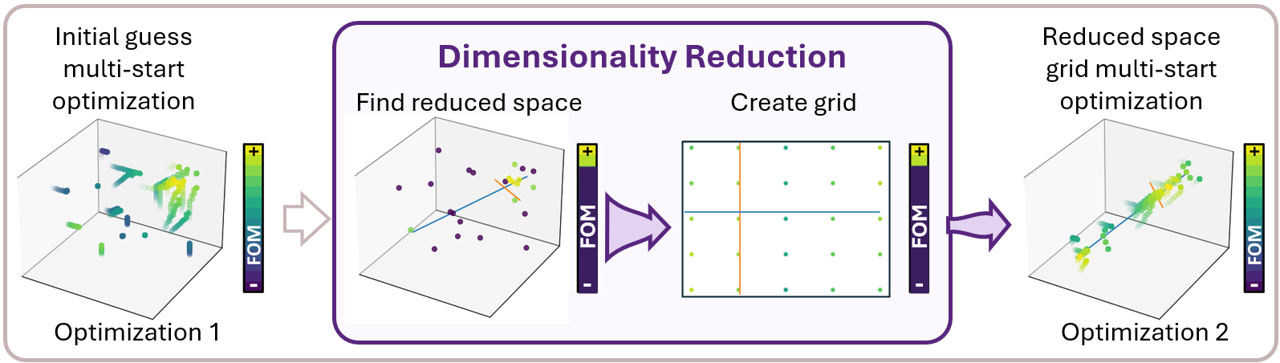
\includegraphics[width=\linewidth]{dr_schema.png}
        \caption{aiirmap dimensionality reduction enhanced design schema. FOM indicates a chosen figure of merit. Figure sourced from \cite{ml-paper}.}
        \label{dr_schema}
    \end{figure}

    The dimensionality reduction implementation is located in \textit{utilities/ml/machine\_learning.py}. This functionality, including the \textit{aiirMapping} object, reflect the schema shown in \autoref{dr_schema}. Functions take a \textit{DataBase} clean and threshold it, apply dimensionality reduction, and then use the reduced space to generate a grid of designs which is projected back into the original design space. This is completed via the \textit{applyDR} function. The exploratory nature of machine learning application led to the further development of so-called "DR investigations". These are sets of multiple dimensionality reduction (DR) runs with differing parameters which are applied to the same input data and saved together in the form of a pickle and pandas dataframe csv. See the code, specifically \textit{investigateDR}, for more info. A wrapper which automatically detects whether a single or multiple/investigation dimensionality reduction is being run is found in \textit{runNewDR}. Some functions for analyzing the reduced space and the reconstruction of data (when datapoints are projected into and then back out of the reduced space) are also provided.  \\         

    
    
    \section{Adding New Simulation Software or Machine Learning Algorithms } \label{new}
    The design philosophy of aiirmap is for it to be a general purpose framework which allows any simulation softwares which can communicate with Python to be coupled to all of the powerful databasing, optimization, machine learning, analysis, visualization, control, etc. capabilities written in Python packages. New simulation softwares can be added, as can new machine learning algorithms. This section will briefly outline the procedures for each.\\

    Adding new simulation softwares into aiirmap will depend highly upon the context. Specifically, how the new software communicates with Python. The main functionality of the new interface is to be able to collect a correctly formatted \textit{DataBase} csv. It is suggested that the user familiarize themselves with the \textit{DataBase} format as described in \autoref{objects} above and in \textit{utilities/databasing.py}. Other functionality may be added, such as run control and/or storage of simulation files but is not required (although the author does suggest run control to allow two-way communication between aiirmap and your software). Interaction with Sentaurus provides all three of these functionalities and may be used as an example, see \autoref{tcad} and \textit{utilities/sReadAndInteract.py} for more information. As the Sentaurus TCAD section outlines, the interaction between Sentaurus and aiirmap is a bit convoluted due to the operational paradigm of Sentaurus, new software implementations may contain many less functions than was required in \textit{sReadAndInteract.py}. Sharing the added software functionality in the github repository is greatly appreciated! Please write a new utility file similar to \textit{sReadAndinteract.py} with the new interface and feel free to add a section to this document outlining its use (locate it in \autoref{softwares}). \\

    Adding new machine learning algorithms into aiirmap can be done two ways. If the new algorithm use is light, exploratory, or time-constrained the user may find it sufficient to implement the new algorithm only within their personal runfiles. On the other hand, if the new algorithm use is substantial, requires standardization, or if the user has the intent to share implementation of the new algorithm involves the creation of new \textit{aiirMapping} variants or addition of similar objects, as the user sees fit. The description of \textit{aiirMapping} objects in \autoref{objects} above and the architecture and comments in \textit{utilities/ml/machine\_learning.py} are pertinent in this case (take care to note how two different dimensionality reduction methods are included). The hope is that a large majority of machine learning algorithms will be able to fit into the \textit{aiirMapping} form factor which would act as a standardized frontispiece for machine learning functionalities which transform the data. Sharing of added functionality in the github repository is greatly appreciated! Please include a brief overview of how to run the new algorithm as a subsection in \autoref{ml}. \\

    
    

    \section{Notes} \label{notes}
    Please be aware of the following points:

    \begin{itemize}
        \item The plotting subfolder (\textit{pldir}) is not used by a great number of the plotting functions. Suggested practice for these functions is to screenshot or save your plots directly from the matplotlib figure window. This course of action allows the user to adjust the aspect ratio and make sure all figure components are visible for each image.
        \item The \textit{amverbose} variable (found in \textit{config.py}) is meant as a global switch to turn off or on extra terminal output. It is only partially implemented. 
    \end{itemize}\\
    
    \section{Publications} \label{pubs}
    The following peer-reviewed publications have utilized the aiirmap framework, listed from newest to oldest:
     
     \begin{itemize}
         \item R.F.H. Hunter, "Next-Generation Multi-Junction Photovoltaic Design Paradigms and Adaptive Optics Techniques for Telecommunications Applications and the Global Energy Transition," Ph.D. Thesis, University of Ottawa, Aug. 2025. 
         \item R.F.H. Hunter \textit{et al.}, "Machine learning enhanced design optimization and knowledge discovery for multi-junction photonic power converters," \textit{Scientific Reports}, Aug. 2025. doi: \url{https://doi.org/10.1038/s41598-025-16408-4} 
         \item M. de Lafontaine \textit{et al.}, "Figures of merit to quantify carrier collection in betavoltaics: Gain and gain efficiency," \textit{Cell Reports Physical Science}, 102789, Aug. 2025. doi: \url{https://doi.org/10.1016/j.xcrp.2025.102789} 
         \item G.P. Forcade \textit{et al.}, “Multi-junction laser power converters exceeding 50\% efficiency in the short wavelength infrared”, \textit{Cell Reports Physical Science}, 6(6):102610, May 2025. doi: \url{https://doi.org/10.1016/j.xcrp.2025.102610}
     \end{itemize}\\

    \noindent
     The following scientific conference presentations (some with proceedings) have utilized the aiirmap framework:

     \begin{itemize}
        \item M. de Lafontaine \textit{et al.}, "Optimizing Tritium Powered GaAs p-i-n and p-n Betavoltaic Cells," \textit{14th International Conference on Tritium Science and Technology}, Ottawa, Canada, 2025.
        \item P. Wilson \textit{et al.}, "Impact of Luminescent Coupling on Multijunction InGaAs Photonic Power Converters under Current Mismatched Conditions in the C-Band," \textit{Photonics North 2025}, Ottawa, Canada, 2025. 
         \item P. Wilson \textit{et al.}, “Quantifying the luminescent coupling process in C-band multi-junction photonic power converters," \textit{Photonics West}, San Fransisco, USA, 2024. 
         \item R.F.H. Hunter, "Using machine learning to optimize multi-junction photonic power converters," \textit{SPIE OPTO 2024}, San Francisco, California, United States, 2024.
         \item K. Hinzer \textit{et al.}, “Multi-junction photonic power converters: AI enhanced design optimization,” \textit{52nd IEEE Photovoltaic Specialists Conference (PVSC)}, Seattle, USA, 2024. 
         \item K. Hinzer \textit{et al.}, “C-band Multi-Junction Photonic Power Converters: AI Techniques for Optimized Designs and Role of Luminescent Coupling," \textit{6th Optical Wireless and Fiber Power Transmission Conference (OWPT)}, Japan, 2024. 
         \item Y. Grinberg \textit{et al.}, “Dimensionality Reduction in Photonics Design – New Methods and Applications,” \textit{Photonics North 2024}, Vancouver, Canada, 2024.
        \item M. de Lafontaine \textit{et al.}, “p-i-n Betavoltaic Cells under 63Ni Irradiation: Quantifying Carrier Collection and Power Output," \textit{52nd IEEE Photovoltaic Specialists Conference (PVSC)}, Seattle, USA, 2024.
        \item G.P. Forcade \textit{et al.}, “High-Performance Multi-Junction C-Band Photonic Power Converters: Calibrated Optoelectronic Model for Next Generation Designs," \textit{50th IEEE Photovoltaic Specialists Conference (PVSC)}, San Juan, Puerto Rico, 2023.
        
     \end{itemize}\\
    
    \noindent
     Users may feel free to add their publications and presentations to the lists. These lists are not considered exhaustive.  \\


    \section{Acknowledgments} \label{ack}
    aiirmap was originally developed as part of the AIIR-Power project \cite{AP_can, AP_ger}. The author is grateful to the agencies which provided funding to the AIIR-Power project and to the members of the consortium for their guidance. While its design diverged significantly over time, aiirmap got its initial inspiration from the project spacemap, developed by AIIR-Power collaborators at the National Research Council of Canada. spacemap is available at \url{https://github.com/NRC-AI4Photonics/spacemap}. This work was completed as part of the author's doctoral studies, the author is grateful to the \href{https://sunlab.ca/}{SUNLAB} research group, to the University of Ottawa, to the Government of Ontario, and to the NSERC CREATE program for funding and support. The aiirmap logo was created with ChatGPT. \\
    

    
    \printbibliography[heading=bibintoc]
\end{document}